%% Creator: Inkscape inkscape 0.92.2, www.inkscape.org
%% PDF/EPS/PS + LaTeX output extension by Johan Engelen, 2010
%% Accompanies image file 'PCLect13p8.pdf' (pdf, eps, ps)
%%
%% To include the image in your LaTeX document, write
%%   \input{<filename>.pdf_tex}
%%  instead of
%%   \includegraphics{<filename>.pdf}
%% To scale the image, write
%%   \def\svgwidth{<desired width>}
%%   \input{<filename>.pdf_tex}
%%  instead of
%%   \includegraphics[width=<desired width>]{<filename>.pdf}
%%
%% Images with a different path to the parent latex file can
%% be accessed with the `import' package (which may need to be
%% installed) using
%%   \usepackage{import}
%% in the preamble, and then including the image with
%%   \import{<path to file>}{<filename>.pdf_tex}
%% Alternatively, one can specify
%%   \graphicspath{{<path to file>/}}
%% 
%% For more information, please see info/svg-inkscape on CTAN:
%%   http://tug.ctan.org/tex-archive/info/svg-inkscape
%%
\begingroup%
  \makeatletter%
  \providecommand\color[2][]{%
    \errmessage{(Inkscape) Color is used for the text in Inkscape, but the package 'color.sty' is not loaded}%
    \renewcommand\color[2][]{}%
  }%
  \providecommand\transparent[1]{%
    \errmessage{(Inkscape) Transparency is used (non-zero) for the text in Inkscape, but the package 'transparent.sty' is not loaded}%
    \renewcommand\transparent[1]{}%
  }%
  \providecommand\rotatebox[2]{#2}%
  \ifx\svgwidth\undefined%
    \setlength{\unitlength}{437.07536316bp}%
    \ifx\svgscale\undefined%
      \relax%
    \else%
      \setlength{\unitlength}{\unitlength * \real{\svgscale}}%
    \fi%
  \else%
    \setlength{\unitlength}{\svgwidth}%
  \fi%
  \global\let\svgwidth\undefined%
  \global\let\svgscale\undefined%
  \makeatother%
  \begin{picture}(1,0.68555644)%
    \put(0,0){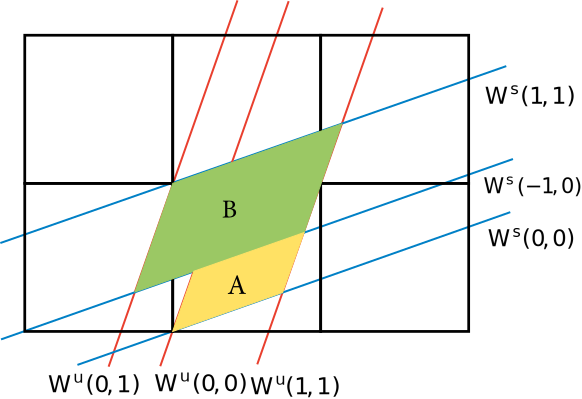
\includegraphics[width=\unitlength,page=1]{PCLect13p8.pdf}}%
    \put(0.83821786,0.26245117){\makebox(0,0)[lb]{\smash{W}}}%
    \put(0.88037687,0.27840246){\makebox(0,0)[lb]{\smash{s}}}%
    \put(0.89701765,0.26245117){\makebox(0,0)[lb]{\smash{(0}}}%
    \put(0.93162325,0.26245117){\makebox(0,0)[lb]{\smash{,}}}%
    \put(0.94889428,0.26245117){\makebox(0,0)[lb]{\smash{0)}}}%
    \put(0.83311117,0.50727046){\makebox(0,0)[lb]{\smash{W}}}%
    \put(0.87674043,0.52381326){\makebox(0,0)[lb]{\smash{s}}}%
    \put(0.89396206,0.50727046){\makebox(0,0)[lb]{\smash{(1}}}%
    \put(0.92977584,0.50727046){\makebox(0,0)[lb]{\smash{,}}}%
    \put(0.94764919,0.50727046){\makebox(0,0)[lb]{\smash{1)}}}%
    \put(0.26507716,0.01331818){\makebox(0,0)[lb]{\smash{W}}}%
    \put(0.30888917,0.02986098){\makebox(0,0)[lb]{\smash{u}}}%
    \put(0.33003861,0.01331818){\makebox(0,0)[lb]{\smash{(0}}}%
    \put(0.36600066,0.01331818){\makebox(0,0)[lb]{\smash{,}}}%
    \put(0.38394951,0.01331818){\makebox(0,0)[lb]{\smash{0)}}}%
    \put(0.08254114,0.01152977){\makebox(0,0)[lb]{\smash{W}}}%
    \put(0.12587645,0.0280725){\makebox(0,0)[lb]{\smash{u}}}%
    \put(0.1467963,0.01152977){\makebox(0,0)[lb]{\smash{(0}}}%
    \put(0.18236796,0.01152977){\makebox(0,0)[lb]{\smash{,}}}%
    \put(0.20012068,0.01152977){\makebox(0,0)[lb]{\smash{1)}}}%
    \put(0.83057203,0.35362439){\makebox(0,0)[lb]{\smash{W}}}%
    \put(0.8694625,0.36839425){\makebox(0,0)[lb]{\smash{s}}}%
    \put(0.88822814,0.35362439){\makebox(0,0)[lb]{\smash{(}}}%
    \put(0.9021929,0.35362439){\makebox(0,0)[lb]{\smash{−}}}%
    \put(0.93012412,0.35362439){\makebox(0,0)[lb]{\smash{1}}}%
    \put(0.94807365,0.35362439){\makebox(0,0)[lb]{\smash{,}}}%
    \put(0.9640133,0.35362439){\makebox(0,0)[lb]{\smash{0)}}}%
    \put(0,0){\includegraphics[width=\unitlength,page=2]{PCLect13p8.pdf}}%
    \put(0.42946843,0.00806193){\makebox(0,0)[lb]{\smash{W}}}%
    \put(0.4730977,0.02460473){\makebox(0,0)[lb]{\smash{u}}}%
    \put(0.49031933,0.00806193){\makebox(0,0)[lb]{\smash{(1}}}%
    \put(0.52613307,0.00806193){\makebox(0,0)[lb]{\smash{,}}}%
    \put(0.54400645,0.00806193){\makebox(0,0)[lb]{\smash{1)}}}%
    \put(0,0){\includegraphics[width=\unitlength,page=3]{PCLect13p8.pdf}}%
  \end{picture}%
\endgroup%
